\chapter{Visuo-proprioceptive spatial discrepancies in proximal body-part}
\label{exp2}
\lhead{Chapter 4. \emph{Visuo-proprioceptive spatial discrepancies in proximal body-part}} 

\section{Introduction}

In the previous chapter, we discussed evidence supporting the hypothesis that multi-sensory visuo-proprioceptive integration mechanisms of proximal body-part plays a role in reach target's spatial encoding. But how exactly is the multi-sensory integration involved in the target's spatial encoding? Let us consider two hypothesis which may plausibly explain the implication of the integration mechanism in reach target's spatial encoding.

%The experiment described in Chapter \ref{exp1} suggests that multi-sensory visuo-proprioceptive integration mechanisms of proximal non-effector body-part play a role in encoding of the spatial information of the reach target. To understand how multi-sensory integration mechanism plays a role in spatial encoding of the reach target, let us consider two hypothesis regarding the integration mechanism.

\begin{figure}[t]
\centering       
    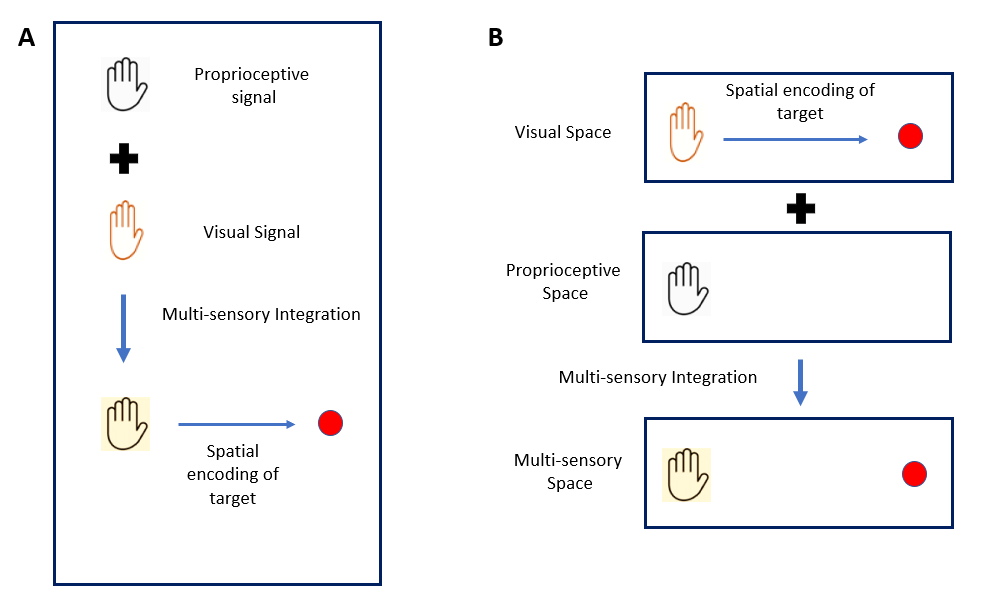
\includegraphics[width=\textwidth, keepaspectratio]{Images/ms_mechanisms.png}
    \caption{Two hypothesis regarding spatial encoding of the reach target. In A), the filled hand denotes the hand position inferred from the multi-sensory integration of visual and proprioceptive uni-sensory signals. The target's spatial location is encoded relative to this inferred hand position. In B) The target's spatial location is encoded relative to the visual signal in the visual space. The visual space is then integrated with the proprioceptive space to construct a multi-sensory representation of body-schema and surrounding peri-personal space.}
    \label{fig:ms-mechanisms}
\end{figure}

\subsection{Spatial encoding with respect to the inferred position of proximal body-part}

One of the mechanisms postulated regarding the specification of body's spatial information in the representation of body (that is, the body schema) is that of visuo-proprioceptive multi-sensory integration. Here, the functional role of multi-sensory integration is to compute reliable estimates of the location of the body part, by integrating the estimates provided by uni-sensory cues on the basis of its reliability and the relevance attributed to the particular modality \cite{limanowski2016integration, noel2018peri, kording2007causal, van1999integration}. In this light, the way multi-sensory integration could be involved in spatial encoding of the reach target is as follows- multi-sensory integration results in the inference of a reliable estimate of proximal body-part's spatial location, and thereafter, the spatial location of the reach target is represented with respect to this inferred spatial location. A schematic of this conjecture is shown in Figure \ref{fig:ms-mechanisms} (A).


\subsection{Spatial encoding with respect to the visual signal of proximal body-part}
An alternative hypothesis is that the spatial encoding of the target could occur with respect to the estimate of the body-part position provided by its visual signal. This visual space, containing a map of visual objects- body part and the target, is then integrated with the proprioceptive space containing a map of proprioceptive objects (see Figure \ref{fig:ms-mechanisms} (B)). The plausibility of this hypothesis is supported by several empirical studies. For instance, the reach target is a visual object, and several studies have shown increases in accuracy of reaching, when visual "landmarks" are in proximity to the reach target \cite<eg.>{conti1980role}, suggesting the occurrence of allocentric encoding of reach target. Furthermore, several studies have also suggested that spatial encoding in allocentric reference frames is used in combination with egocentric representation \cite{byrne2010interactions, schutz2013gaze}, although the literature here refers to eye-centered egocentric representation. Nevertheless, it is plausible that the spatial encoding of visual target is with respect to the visual information, and this visual space is then integrated with proprioceptive space, to construct a multi-sensory representation of space which is characteristic of peri-personal space representation. 


\section{Experiment 2}

To test for these competing hypothesis, we conducted an experiment in which we manipulated the spatial discrepancy between the actual position of the non-action target proximal hand and its visual input, by spatially displacing the visually rendered hand in an Immersive Virtual Reality environment. The objective of this experiment was to understand how reach target location estimation was affected by the spatial discrepancy in the estimates provided by visual and proprioceptive inputs of the body-part (non-action hand) proximal to the target. We also aimed to qualitatively compare which of the mechanistic hypotheses described above explains the the reach accuracy results. If the inferred position of the proximal hand systematically affects the target location estimation, it would suggest that Hypothesis 1 may be the multi-sensory mechanism that could underlie body-proximal reach target spatial encoding. On the other hand, if the proximity to the visual hand systematically affects the target location estimation, Hypothesis 2 may be the mechanism underlying the reach target spatial encoding.


\subsection{Method}

\subsubsection{Participants}
Nineteen right-handed subjects(2 Females, Mean age = 22.68, Range = 18-33) were recruited to participate in the experiment. All participants reported normal or corrected to normal vision. They were naive to the purpose of the experiment and the experimental procedure, and had provided written consent to participate in the study according to the norms approved by the Institute Ethics Committee (IEC) of Indian Institute of Technology, Kanpur. 

\subsubsection{Materials and Apparatus}
The participants sat across a table with surface area dimensions of 120cm x 50cm. Two coin-shaped docks (2.5 cm diameter) were attached to the table with a distance of 46 cm between them at the center of the table. A cylindrical barrier of 2.5cm height was attached around the right dock. The participant sat with their arms resting comfortably on the table, with the right and left docks serving as resting positions for the right and left index fingers respectively. Hand motion and position was tracked with Ultraleap Leap Motion Controller. The virtual reality environment was displayed on Oculus Rift S Head-mounted Display, and developed using Unity Game Engine. The virtual scene consisted of a virtual table situated in a black room. The virtual table was spatially aligned to the physical table at which the participant sat. The target of the reach was a red dot of 0.5cm in diameter. 

\subsubsection{Procedure}

The experiment began with a calibration session, similar to the session performed in Experiment 1 (Refer Chapter \ref{exp1}). The experiment consisted of 5 Experimental blocks which were interleaved with filler blocks. For the experimental blocks, the participants were instructed to place their left hand on the dock, whereas for the filler blocks, the left hand was placed on the lap. The experimental blocks differed in the position at which the left hand was rendered visually in the virtual scene. The visual rendering of the left hand, henceforth termed as the visual hand, was positioned at five locations - congruent to the left hand placed at the left dock (henceforth termed as the proprioceptive hand), 5.75cm, and 11.50cm to the right of proprioceptive hand, and 5.75cm and 11.50cm to the left of the proprioceptive hand. The order of the experimental blocks was counterbalanced across participants using Latin Square counterbalancing design. 

\begin{figure}
\centering       
    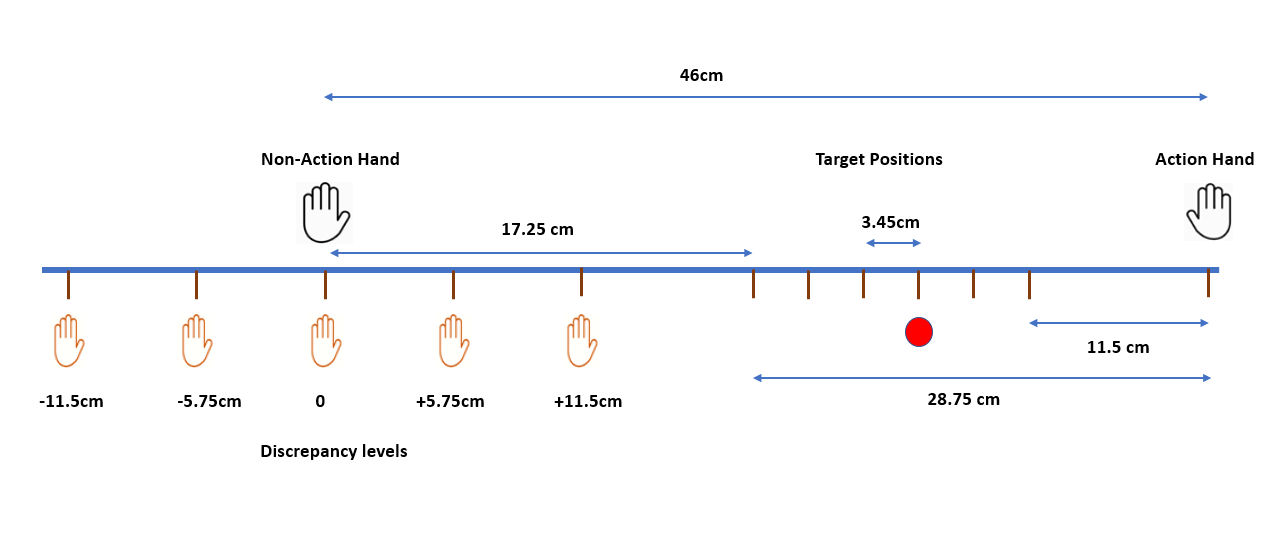
\includegraphics[width=\textwidth, keepaspectratio]{Images/exp2_task.png}
    \caption{Experimental Setup}
    \label{fig:exp2-task}
\end{figure}

Within each block, the target appeared at one of the following 6 locations along the axis joining the two docks, at a distance of  28.75, 25.30, 21.85, 18.40, 14.95, and 11.50 cm from the action hand (see Figure \ref{fig:exp2-task}). The experimental blocks each consisted of 10 x 6 (target positions) = 60 trials, while the filler blocks consisted of 5 trials each. 

The task performed by the participant was same as that of experiment 1. Each trial was initiated by bringing the right index finger on the right dock. On an audio cue, the target appeared at one of the above mentioned target locations, after which the participant attempted to make contact with the target with their right index position. The trial ended with the disappearance of the target after the contact was detected between the table and the right index finger. The participant brought the right hand back to the right dock to initiate the next trial. Throughout the course of the experiment, the right (action hand) was rendered invisible. 


\subsubsection{Experimental Design}

The accuracy of the spatial encoding of the target in reach action was operationalized as \textit{reach error}, which was computed as the difference between the actual location of the target and the estimated location of the target, indicated by the participant by the end-point of the reach action. Positive reach error indicates that the relative to the actual position of the target, the estimate of the target location is in the direction towards the action hand. On the other hand, negative reach error indicates that target location estimate is to the left of the actual target location in the direction of the the non-action hand. 

The experiment was set-up in a within-subjects experimental design, with reach error as the dependent variable. The two independent variables that were experimentally manipulated were - i) The non-action hand visuo-proprioceptive spatial discrepancy, that is, the distance between the actual position of the hand (proprioceptive hand) and the visual rendering of the hand (visual hand), and ii) The distance between the initial position of the action hand and target (AHT). 

\subsection{Data Analysis}

\begin{table}[t]
\centering
\resizebox{\textwidth}{!}{
\begin{tabular}{llrr}
  \hline
  Model & Fixed effect & AIC & BIC \\
  \hline
  Null Model & None &	28746 &	28779 \\
  Discrepancy Model & Discrepancy	& 28731	& 28770 \\
  AHT Model & AHT &	28698 &	28737 \\
  Additive Model & Discrepancy + AHT	& 28683	& 28729 \\
  \textbf{Interaction Model} & \textbf{Discrepancy + AHT + (Discrepancy * AHT)} & \textbf{28666} & \textbf{28719}\\
   \hline
\end{tabular}}
\caption{AIC and BIC Values for fitted Linear Mixed Effect models. Random effects of all models consisted of intercepts for subjects and by-subject random slopes for effect of discrepancy ( $1 + discrepancy | subject$ ). The interaction model has the lowest AIC and BIC value. }
\label{table:lme-models}
\end{table}

  
 


To understand the effect of visuo-proprioceptive spatial discrepancy on the reach error, we performed a linear mixed effects analysis using the \emph{lme4} ~\cite{bates2014fitting} and \emph{lmerTest} packages in R. We considered visuo- proprioceptive spatial discrepancy and the distance from action hand (AHT) as fixed effects in our models. Random effects of all models that we fit consisted of intercepts for the subjects and by-subject random slopes for the effect of discrepancy. Table \ref{table:lme-models} states the fixed effects of the various fitted models and their Akaike information criterion (AIC) and Bayesian Information Criteria (BIC) values. Likelihood Ratio Test was performed to compare the models and as a criteria for model selection. Refer Appendix \ref{App-exp2-analysis} for the results of the Likelihood Ratio test. 

The AIC, BIC, and the results of the Likelihood Ratio Test reveal that the best fit model consisted of discrepancy and AHT as the fixed effects, along with an interaction between the two predictors (see Table \ref{table:lme-bestfit-fixedeffect}). There were no obvious deviations from homoscedasticity and normality on the basis of visual inspection of residual plots (See Figure \ref{fig:lme-residual} and Figure \ref{fig:lme-norm}). Furthermore, we checked for multi-collinearity between the predictors by using Variance Inflation Factor (VIF) as a measure of collinearity using the package \emph{performance} in R. The results show low correlation (VIF < 2) between the fixed effect terms of the best-fit model (see Table \ref{table:collinearity}).

Moreover, we performed bootstrapping to get credible confidence intervals at 95\% for the estimates of the fixed effects (see Table \ref{Table:Bootstrapped estimates}). None of the confidence intervals for the fixed effects contain the value 0, which further supports the significance of the effects of the three predictors (discrepancy, AHT, and interaction) on the reach error. 

Thus, the results of the Linear Mixed Effects analysis shows that the interaction between the spatial discrepancy between the visual and proprioceptive inputs of the proximal non-action hand and the distance between the target and the action hand has a statistically significant effect on reach error. This suggests that the way visuo-proprioceptive spatial discrepancy of proximal non-action hand affects the target estimation depends upon the distance of the target from the the action hand. Therefore, to interpret the results, we will consider the effect of visuo-proprioceptive discrepancy separately at different distances of target from the action hand. 



\subsection{Support for visual anchoring mechanism}
\begin{figure}[t]
\centering       
    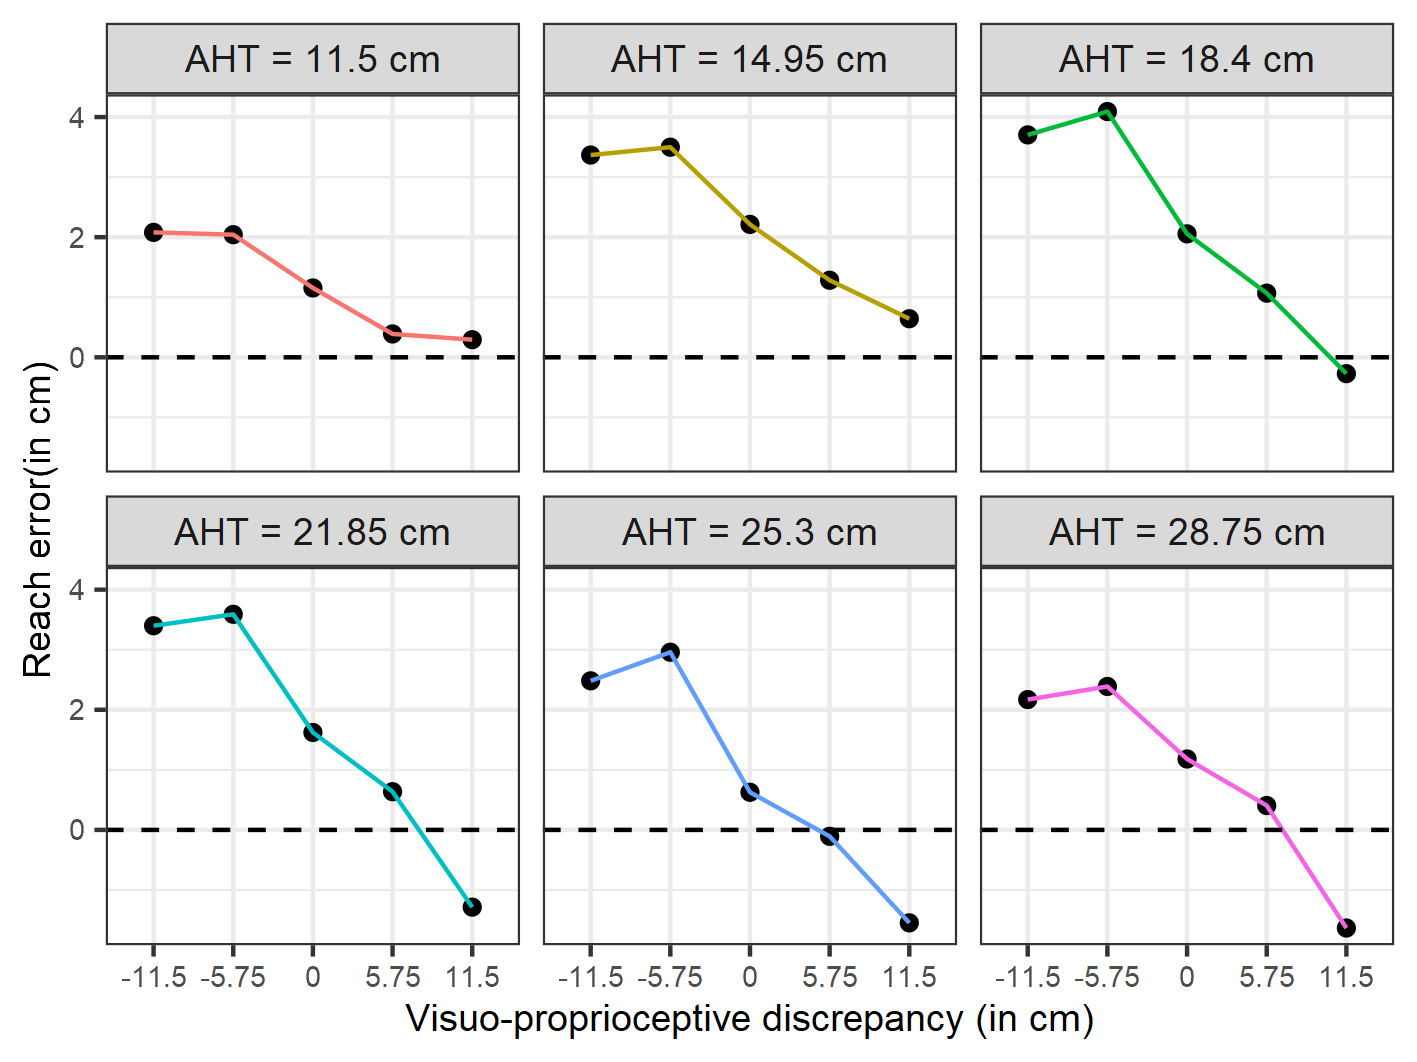
\includegraphics[scale=1]{Images/exp2_results2.png}
    \caption{Reach error as a function of spatial discrepancy between the position of visual hand and the position of actual (proprioceptive) non-action hand. Each panel shows the distance between the target and the initial position of the action hand (AHT). Negative reach error indicates that the estimation of the target location was in the direction of the non-action hand towards the left, while positive reach error indicates that the location of the target was estimated in the direction of action hand towards the right of the actual location of the target.}
    \label{fig:exp2_re-aht}
\end{figure}

Figure \ref{fig:exp2_re-aht} shows the effect of visuo-proprioceptive spatial discrepancy of proximal non-action hand on reach error, at different reach distances, that is, distance between the target and the initial position of the action hand. 

Since, the location of the proprioceptive signal is fixed according to the design of the experiment, the values of visuo-proprioceptive discrepancy also may be interpreted as different positions of the visual hand. The results in Figure \ref{fig:exp2_re-aht} show that there is a general underestimation (reach error is positive), when the target is closer to the action hand (Panel AHT = 11.5, 14.95, 18.4). However, as the visual hand is rendered closer to the target, the reach error decreases and the target estimation is more accurate. However, as the distance between the target and the action hand increases (Panels 21.85, 25.3, 28.75), the reach error is negative when the visual hand is rendered very close to the target (Discrepancy = +11.5cm). This suggests that it is not the accuracy that is improving as the visual hand is placed closer to the target, rather the estimate of the target's location is "pulled" towards the proximal non-action hand, as the distance between the visual hand and target decreases.

Overall, the results suggest that it is not the visuo-proprioceptive discrepancy itself that is affecting the target's location estimation, since that would have displayed a convex or a concave curve, with same magnitudes of discrepancy showing similar reach errors. Rather, the proximity of the visual hand to the target biases the estimation of the target in its direction, suggesting that the spatial encoding of the target may be with respect to the visual information of the body part in proximity.

These results seem to contradict the hypothesis that the spatial encoding of the target is with respect to the position of the body-part estimated as a result of multi-sensory integration inference mechanism. 

\subsection{Lack of support for Bayesian Causal Inference Mechanism}

The competing hypothesis that we will now consider is that the spatial information of the reach target is encoded with respect to the position of the proximal body-part which is estimated as a result of multi-sensory integration process. One of the models of multi-sensory integration is the \textit{Bayesian Causal Inference Model}. This model specifies how noisy uni-sensory signals are weighted based on the probability that the signals arose from the same source, and then integrated according to Bayesian Inference \cite{kording2007causal, meijer2020computational}. Previous literature suggests that this model can reasonably explain how position of the body part is estimated from noisy visual and proprioceptive signals \cite{noel2018peri, fossataro2020immersive}. We implemented the model similar to the implementation by \citeA{fossataro2020immersive} to estimate the position of the non-action hand from the visual and proprioceptive signal positions as specified by the experimental manipulations described in the above experiment.

According to the model, the uni-sensory information is modeled as a probability distribution, specifying the probability at all possible locations that the uni-sensory object is present at that particular location. In this implementation, the visual and the proprioceptive signals are assumed to follow a Gaussian distribution, centered at the veridical location of the signal (specified by the experimental manipulation), with variance indicative of the sensory noise. In our implementation, we set the value of visual precision (inverse of variance) as 0.97, and the value of proprioceptive precision as 2.1, on the basis of results found by \citeA{noel2018peri}. The third parameter of the model is $P_\pi$, which represents the "prior" beliefs that the visual and proprioceptive signals belong to the same source. We set the value of $P_\pi = 0.5$ in our implementation.

The complete model is specified as - 

\begin{align*}   
    P(hp | x_v, x_p) 
    &= \Sigma_{c=own,diff} P(hp | x_v, x_p, C = c) P(C = c | x_v,x_p ) \\ 
    &= P(hp | x_v, x_p, C = own) P(C = own | x_v,x_p ) \\
    &+ P(hp | x_v, x_p, C = diff) P(C = diff | x_v,x_p )
\end{align*}

where, $P(hp | x_v, x_p) $ is the probability of inferred location of the non-action hand, given the uni-sensory signals $x_v$ and $x_p$. $C=own$ refers to the situation where the source of the two signals is same, while $C=diff$ refers to the situation where the source of the two signals is different.  When $C=own$ , $P(hp | x_v, x_p, C = own)$ is the Gaussian posterior distribution, centered at the average of the uni-sensory signals, with a variance equal to the inverse of the sum of the precision of the uni-sensory signals. When $C=diff$ , $P(hp | x_v, x_p, C = diff)$ is the probability distribution relying only on proprioceptive signal - Gaussian centered at mean of proprioceptive signal, with the proprioceptive signal noise as its variance. The weighing factors $P(C = own | x_v,x_p )$ and $P(C = own | x_v,x_p )$ specify the probabilities that the two uni-sensory signals arise from the "own" hand or "different" sources conditional on the uni-sensory signals. 

\begin{figure}[t]
\centering       
    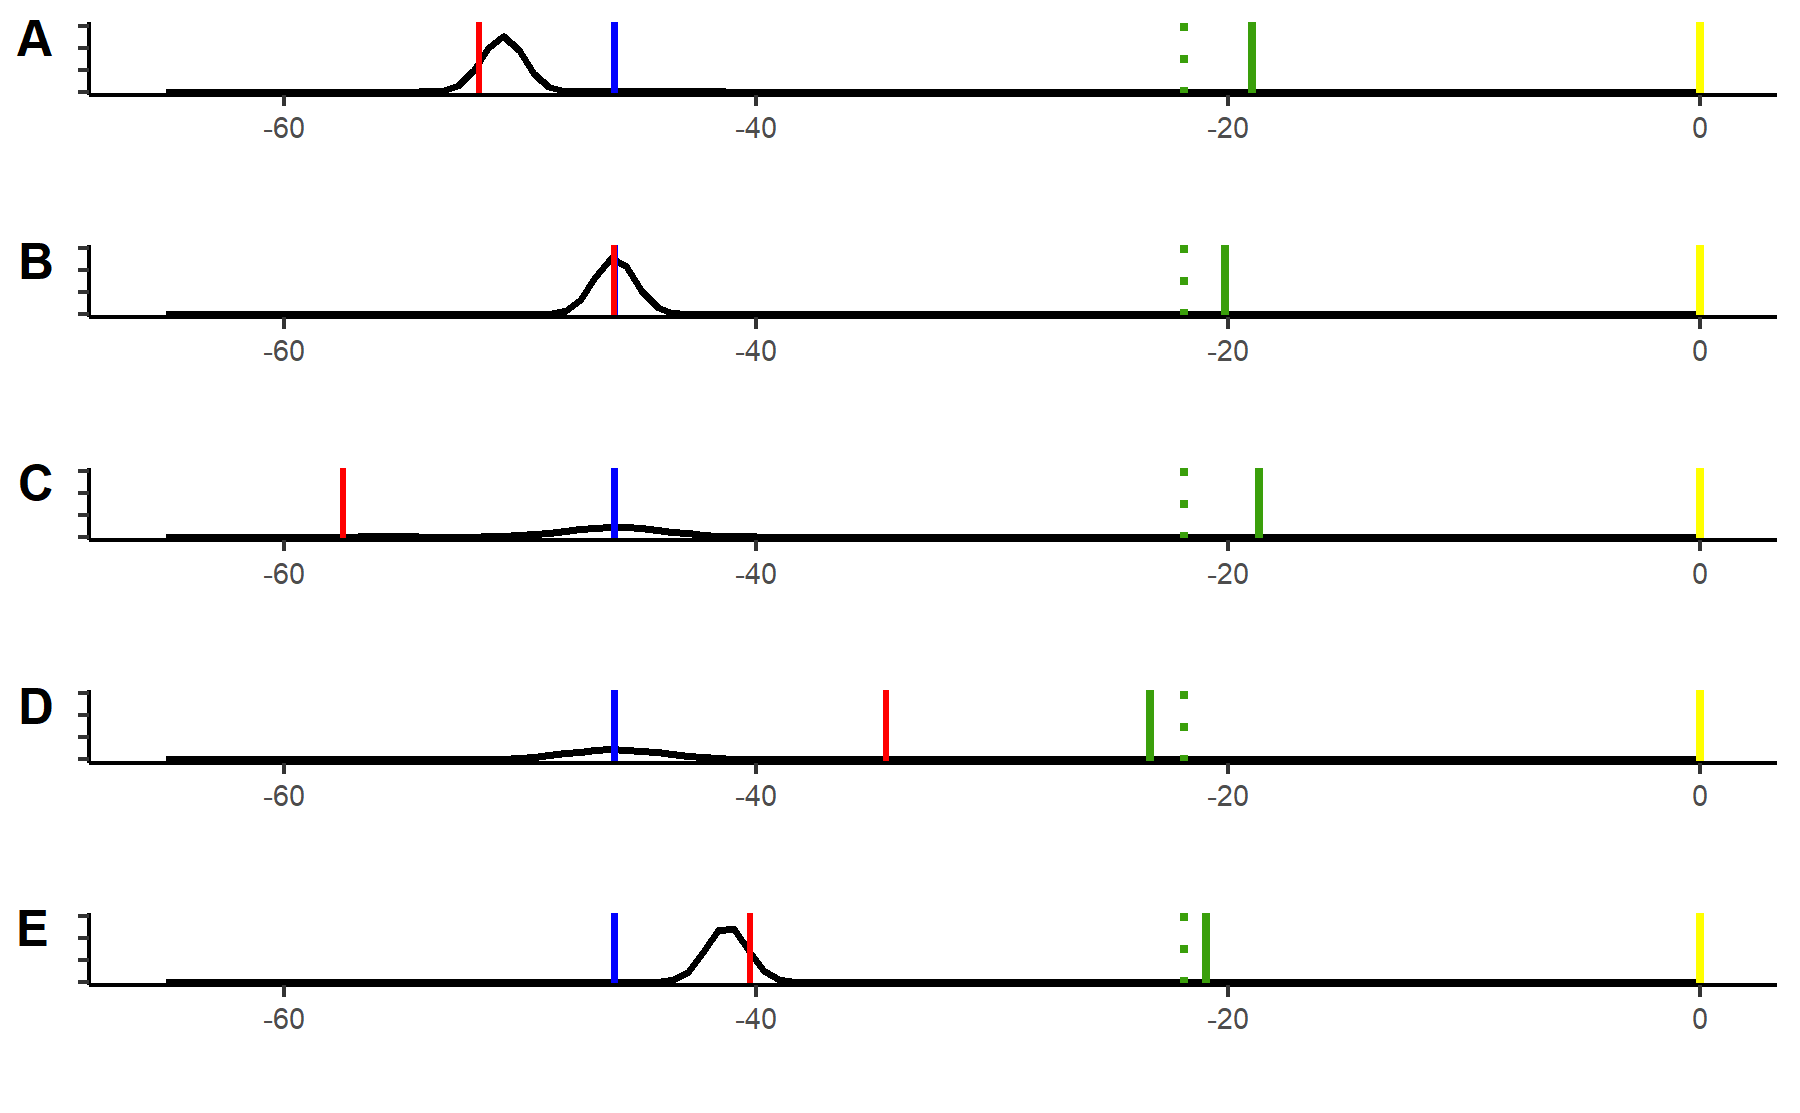
\includegraphics[width=\textwidth, keepaspectratio]{Images/bci_plot2.png}
    \caption{Estimated target location for Target Location = 21.85 cm, for different proximal hand's inferred positions according to the Bayesian Causal Inference Model. The red line indicates position of the visual signal of the proximal hand, while the blue line indicates the position of the proprioceptive signal, that is, the location of the placement of the real hand. The black curve indicates the probability density function denoting the probability of the location of the hand, as postulated by the multi-sensory integration process specified in the Bayesian Causal Inference Model. The mode of the distribution indicates the inferred position of the hand. The green dotted line indicates the veridical position of the reach target, while the solid green line indicates the (average) located estimated by the subjects. The yellow line indicates the initial position of the action hand. Panels A to E are ordered by the increasing proximity of the inferred hand position to the reach target, As seen in the figure, there is no systematic effect of proximity between the target and inferred hand position, and the target location estimation. }
    \label{fig:bci-plot2}
\end{figure}

We implemented this model to derive the probability distributions of non-action hand position at different levels of visuo-proprioceptive discrepancy. Figure \ref{fig:bci-plot2} shows these distributions with panels ordered according to the mode of the inferred hand position. Reach target veridical position at 21.85 cm from action hand and its average estimated position is also plotted (for other target positions, refer to Appendix \ref{App-bci-plots}). We observe that in the case of a high magnitude of visuo-proprioceptive discrepancy (Panel C and D, discrepancy = -11.5cm and +11.5cm), the mode of the inferred hand position is situated at the position of the proprioceptive hand. This is due to high probability attributed to the source of the uni-sensory signals being different (C = diff), due to the higher magnitude of spatial discrepancy between them. On the other hand, when the visuo-proprioceptive signals are relatively close (Panel A and E, discrepancy = -5.75cm and +5.75cm), we observe that the mode of the inferred hand position is shifted towards the visual hand. This is due to the high probability attributed to (C = own) and higher precision of visual signal. 

Qualitative inspection of the figure reveals that there is no systematic effect of the inferred position of the non-action hand on the reach target location estimation. In particular, consider Panel C and D. While the inferred position of the non-action hand is same in both cases, along with same uncertainty associated with the probability distribution, we observe differences in estimates for the reach target location. No systematic effect of inferred hand position is observed at other target positions as well (see Appendix \ref{App-bci-plots}). 

Therefore, the results of the experiment do not support the hypothesis that spatial encoding of the reach target occurs with respect to the inferred position of proximal body-part according to the Bayesian Causal Inference Model. On the other hand, the spatial encoding of reach target can be explained by encoding of the target's spatial information with respect to the visual signals of the proximal body-part, based on our results. 













